\documentclass[10pt]{article} 
\usepackage{enumitem}
\usepackage{graphicx}
\usepackage{subfig}
\usepackage[margin=1in]{geometry}
\usepackage{amsmath}
\usepackage{dirtytalk}
\usepackage{color}
\usepackage[numbers]{natbib}
\title{Assignment 2: Patterns\\
      Squeezing it}
\author{Shrestha Ghosh (2567717, s8shghos@stud.uni-saarland.de)}
\begin{document}
\maketitle
\section{Introduction: Sequential Pattern Mining}
\par We are often required to characterize or summarize a large database of transactions which motivates the practice of pattern mining. While frequent pattern mining is an efficient pattern mining approach, made efficient due to the monotonic property of frequency of itemsets, frequency in itself is not a very useful measure of interest. Hence, the patterns obtained using this measure, the Apriori method and the likes do not exhibit any special property of the data. Lower frequency thresholds mined exponential patterns which are often redundant (pattern-explosion) and higher frequency thresholds yielded common and already known patterns. Two alternate measures of interest are presented by~\citet{tatti2012long} through their method named SQS and~\citet{fowkes2016subsequence} in their model named ISM.
%\par How can we perform pattern mining? Why is Apriori not sufficient?
%\par Analyze two approaches - an MDL based encoding scheme and a generative model

\section{The MDL approach - SQS}
\par SQS is based on the minimum description length (MDL) principle with the argument that the set of patterns which best summarize (encode) a model are also the most informative and less redundant patterns. Pattern in sequential mining is considered to be a serial episode. The reduction in redundancy in patterns mined using frequency measure is evidently absent from the SQS generated candidates if we compare the tables in Fig.~\ref{comparejmlr}. A code table (CT) is the model which describes the patterns and their associated codes, gap and non-gap codes. SQS uses MDL principle to score each model on number of bits needed to describe the model plus the number of bits required to store data in encoded form. MDL scoring is straight-forward - number of bits required for patterns codes, gap codes and non-gap codes are log dependent on their relative frequency (by Shannon's information entropy) and the entire database requires respective code bits multiplied with its usage (frequency of the code used). We can understand that at the heart of the scoring lies the frequency measure. But, when used in a more sophisticated fashion, here in an information theoretic approach, we obtain patterns which optimize the score 
\begin{equation}
L(D,M) = L(M) + L(D|M)
\end{equation} 
and hence these patterns are more meaningful than just being \textit{frequent}. These patterns belonging to a model $M$, which in this case is a CT, optimally summarize the data $D$. So, we see that an assumption on the model is made. Instead of searching the entire space of models the authors consider only the subspace of CTs. Since a given set of patterns (or a CT) can be used in multiple ways to cover a database. For e.g., in Fig.~\ref{ctsample}, $CT_2$ is derived from a minimal set of pattern set $P={(a), (b), (c), (d), (abc), (da)}$ another cover for data D could have been {$(a)(b)(d(c)a)(d(b)a)(abc)$}. Thus, the score to be optimized is more specifically defined as
\begin{equation}
L(CT, D) = L(CT|C) + L(D|CT)
\end{equation}
where, an optimized $L(CT|C)$ score means finding the best cover $C$ for a given set of patterns and using the CT for that $C$.

\begin{figure*}
%\begin{figure}
\begin{center}
\subfloat[Comparing patterns: \textit{Top Table} (referred from~\citet{lam2014mining}) shows the 20 most frequent non-singleton closed sequential patterns from the JMLR abstracts datasets. \textit{Bottom Table} (referred from~\citet{tatti2012long}) as the heading suggests shows the top 10 patterns returned by SQS-SEARCH.
\label{comparejmlr}]{%
		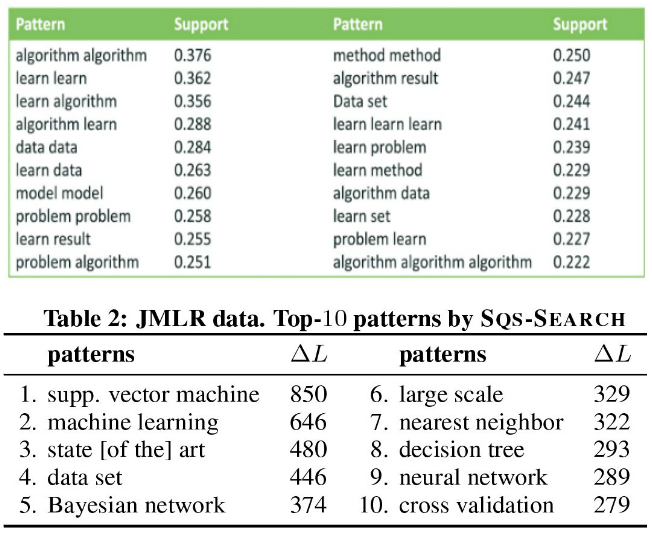
\includegraphics[width=8cm]{jmlr_compare.jpg}
		}
		\hspace{0.2cm}
%\caption{Comparing patterns: \textit{Top Table} (referred from~\citet{lam2014mining}) shows the 20 most frequent non-singleton closed sequential patterns from the JMLR abstracts datasets. \textit{Bottom Table} (referred from~\citet{tatti2012long}) as the heading suggests shows the top 10 patterns returned by SQS-SEARCH.}
%\label{comparejmlr}
%\begin{figure}
%\begin{center}
\subfloat[Toy examples of possible encodings referred from~\citet{tatti2012long}\label{ctsample}]{%
		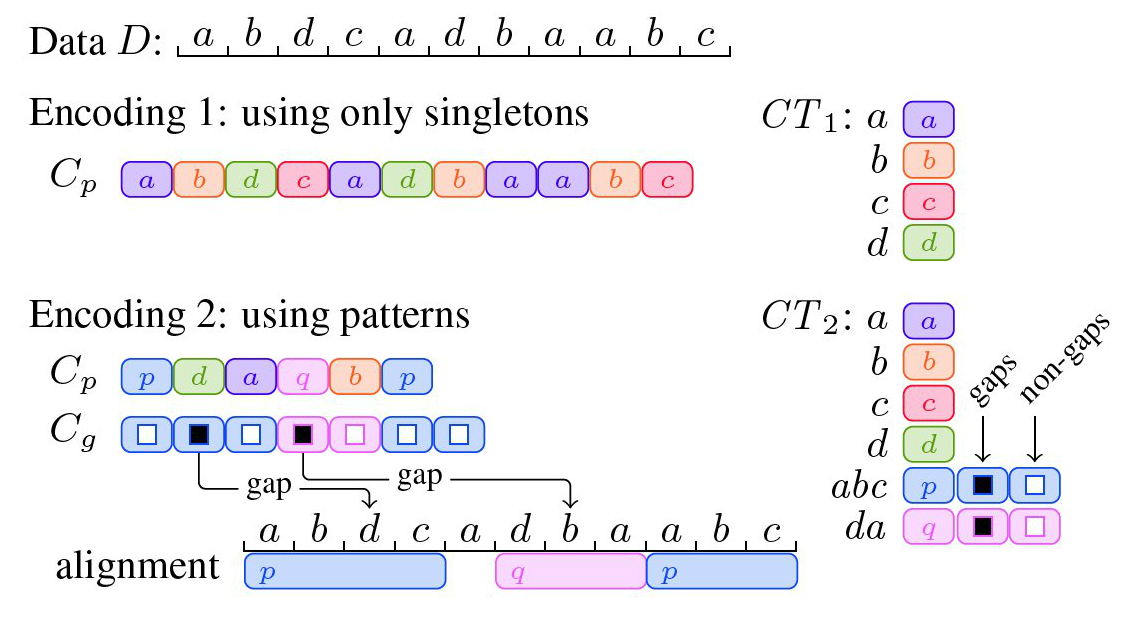
\includegraphics[width=6.5cm]{CTsample.jpg}
		}
%\caption{Toy examples of possible encodings referred from~\citet{tatti2012long}}
%\label{ctsample}
%\end{center}
%\end{figure}
\end{center}
%\end{figure}
\end{figure*}

\par SQS has to now find that CT which is optimal for the optimal cover C of the data in order to get the optimal MDL score. While punishing gaps helps finding better alignments for a cover, the validity of an alignment is based on the assumption that all active windows must be disjoint. Disjoint windows may not be able to identify collocated events which occur as interleaved pattern in the database. For example in $CT_2$ of Fig.~\ref{ctsample}, the code sequence fails to recognize the first occurrence of the pattern $da$ because it's window overlaps with the pattern $abc$. If our application is such that we would like to find collocated events then disjoint window assumption does not hold.

\par For a comprehensive comparison method is presented by~\citet{lam2014mining} where models are compared based on four criteria - pattern interpretability, run time, compression and classification accuracy. Since the algorithm presented is based on MDL principle and considers interleaving patterns, it can be fairly compared with SQS. The comparison between SQS and the proposed models is not provided for classification accuracy. SQS is beaten in run time and recall and in compressibility by a small margin.  
%\par ~\citet{tatti2012long} approach allows gap encoding and punishes long gaps
%\par Ranking patterns 
%\par Importance of setting a support threshold
%\par redundant and spurious patterns

\section{The generative model - ISM}
\par In the previous section we saw models which CTs and optimize an MDL based score for a given sequential database.~\citet{fowkes2016subsequence} important contribution is developing a generative model of the database conditioned on the patterns, \emph{i.e.,}
\begin{equation}\label{ismopt}
p(X|\Pi,\mathcal{I})
\end{equation} The algorithm uses expectation maximization (EM) framework starting with $\mathcal{I}$ and $\Pi$ initialized to singletons and their relative frequency, respectively. The algorithm iteratively adds best candidate sequence by combining existing sequences in $\mathcal{I}$ and optimizes $\Pi$ based on new $\mathcal{I}$ removing any old sequence which may not be useful in generating data $X$ till convergence. 
\par The model maximizes the probability that $\mathcal{I}$ generates $X$ given $\Pi$ by generating a non-overlapping multiset cover of $X$. The objective function in ISM, which is to optimize Equation~\eqref{ismopt}, requires ISM to find the optimal cover for the given set of patterns. Then EM is used iteratively to add new sequences until Equation~\eqref{ismopt} can no longer be improved. Same as in SQS, ISM prunes the older sequences which are no longer required to explain the data because of the new better patterns added to $\mathcal{I}$. However, it is to be noted that ISM does not consider punishing gaps in the sequences. In ISM, multiset of a pattern is same as the window of of a pattern in SQS. Therefore, for finding the cover, ISM needs to find the the optimal number of windows of each pattern in the pattern set $\mathcal{I}$ given the probability of occurrence of number of windows of each patterns in $\Pi$. 

\par ISM does not place any constraints on the size of the window of a pattern. Let us analyze the greedy algorithm used for building the cover by maximizing a submodular function. We consider the same data in~\ref{ctsample}, \emph{i.e.,} $X=abdcadbaabc$ (consider data has a single sequence) and start with all singletons and suppose we find the new candidate sequences say, {\color{blue}$(ab)$} and {\color{green}$(da)$} using the greedy algorithm. Subsequently {\color{red}$(abc)$} is be added because the greedy algorithm gets higher score for a multiset ${\color{red}abc}{\color{green}da}{\color{green}da}b{\color{red}abc}$ than an overlapping multiset ${\color{red}abc}{\color{blue}ab}{\color{green}da}{\color{blue}ab}{\color{green}da}{\color{red}abc}{\color{blue}ab}$. As mentioned in the text, any singletons removed are reseeded when necessary. Thus we find interleaving patterns as well as remove uninteresting ones like  {\color{blue}ab}. The authors explain multiplicity for a single item. But, the multiplicity for a pattern is not properly defined. Is it in terms of minimal window (\#(abc) in X = 2) or fixed window (\#(abc) in X = 3 for fixed window 4) is not clear. And, maybe the gaps are implicitly taken care of by the cover if minimal windows are selected. For example pattern $(ac)$ in the above sequence X has large gaps as compared to the pattern $(da)$. It remains to be seen if in the candidate generation algorithm (Algorithm 4) $(da)$ is placed above $(ac)$ in the priority queue. This might explain ISM's performance despite of ignoring gap penalty.

\par The performance measuring the pattern redundancy there are related patterns like (large scale, high dimension) and (machine learn, learn algorithm) returned by SQS though all returned patterns are highly interpretable and related to the machine learning context. While ISM returns diverse patterns, patterns like (first second, wide range, wide varieti, turn out) are general patterns. Whether edit distances and common subsequence frequency are good measures of redundancy is debatable - consider two patterns 'principle of MDL' and 'principal component' which are very different concepts with low edit distance and common subsequence. Classification accuracy is still a fair measure between the models since classification accuracy tests the applicability of the patterns generated and not the patterns themselves which makes sense because the generation procedure of ISM and SQS is very different. Pattern interleaving comparison done between different models (SQS, ISM and GoKrimp) is unfair since it is already known that SQS does not return interleaving patterns. If we consider fair competition GoKrimp has better recall than ISM. On similar argument pattern spuriousness is a validation check for ISM and is not a fair platform for comparison. Also, how the generative model used to sample 10.000 sequences was constructed is not explained.

\par Since SQS is based on MDL principle where the class of models considered can be anything (SQS specifically considers CTs), we could use MDL principle to encode ISM models which would then entail calculating the number of bits to store set of patterns $\mathcal{I}$, the probability vector of multiplicity $\Pi$ to calculate $L(M)$. However, we arrive at a roadblock for calculating $L(X|M)$ in ISM. Being a probabilistic model, ISM at no point actually generates the dataset X. The distribution from which X is sampled is also never constructed since we only require the cardinality of this distribution which is approximated. ISM gives us the multiset of sequences which can best generate X, hence, if the set of patterns $\mathcal{I}$ is considered an encoding of $X$, it is lossy, since we cannot exactly get back X. This is same as having the CT for a database in SQS with the pattern multiplicities but never getting the generated code $C_p$. Due to lack of common scoring ISM in the current state cannot be directly compared to SQS regarding the quality of patterns generated.
  
%allowing interleaving patterns. What were we missing out without interleaving?
%\par Gap penalties not explored.
%\par Is model complexity truly compared? How do encode the generative model?
%Since in MDL the length is length of data given model plus model. ISM complexity in terms of MDL is length of data encoded given the patterns plus the length to encode the model generating those patterns. Is Code Table for MDL same as the generative model for ISM?
%
%\par The results showing top patterns are common for that particular dataset. How are new  patterns within dataset learned? Say ML techniques have moved from Naive Bayes to SVM ?

\section{How can we speed up SQUISH and SQS-Search?}
\par An extension of SQS is proposed by~\citet{bhattacharyya2017efficiently} named SQUISH. Based on MDL principle, SQUISH mines interleaving patterns, patterns with multiple events at the same time - all patterns have budgeted gaps. This allows for a richer description of the sequential data in a succinct format. If we see the runtime of SQUISH we will observe that the steep decrease in $L(CT,D)$ occurs almost immediately and then the runtime saturates after 200 sec without any significant gain in the encoded length. This implies that SQUISH finds the most effective patterns first and as time progresses the patterns found are less effective. The rate of change of $L(CT,D)$ is rapid at first and slowly approaches zero in the later stage. Firstly, we could set a change threshold in outermost loop of SQUISH where instead of iterating till no changes, we iterate till the rate of change goes below a certain threshold. 

\par The candidate generation heuristic considers every possible extension then sort and return the best extension. If the EM method of candidate generation is adopted, then we consider every extension $Y$ of $X$ in order of decreasing support of $XY$ in the database and continue to next $Y$ only if there is no improvement. Speeding up the heuristic estimate can speed up both SQUISH and SQS methods.         

\par The number of database passes in SQS can also be reduced during the recursive testing a newly added candidate with adding gap intermediates. The number of recursive calls can be reduced if testing is done on gap items such that it is not a superset of an already been pruned pattern from past prune iterations. This will then require that we keep a tab of pruned patterns. 

\bibliographystyle{plainnat}
\bibliography{report2}
\end{document}